\documentclass[11pt,a4paper]{article}

\usepackage[utf8]{inputenc}
\usepackage[T1]{fontenc}
\usepackage[spanish,es-nodecimaldot]{babel}
\usepackage{lmodern}

\usepackage{graphicx}
\usepackage{geometry}
\usepackage{array}
\usepackage{amsmath}
\usepackage{titlesec}
\usepackage{hyperref}
\usepackage{fancyhdr}

\usepackage{booktabs}
\usepackage{float}

\fancyhf{}

\fancyhead[L]{\small\textit{Universidad Nacional de Ingeniería}}
\fancyhead[R]{\small\textit{2026--II}}
\renewcommand{\headrulewidth}{0.4pt}
\fancyfoot[C]{\thepage}

\geometry{
    top=2.2cm,
    bottom=1.5cm,
    left=2.5cm,
    right=2.5cm,
    headheight=14pt,
    headsep=0.5cm
}

\setlength{\parindent}{0pt}
\setlength{\parskip}{0.5em}
\pagestyle{plain}
\setcounter{secnumdepth}{2}
\setcounter{tocdepth}{2}
\addto\captionsspanish{%
    \renewcommand{\contentsname}{Contenido}%
}
\hypersetup{
    colorlinks=true,
    linkcolor=black,
    citecolor=black,
    urlcolor=blue
}

\titlespacing*{\subsection}
    {0.6cm}
    {1.5em}
    {0.8em} 

\newenvironment{subsectionbody}
{%
    \begin{list}{}{%
        \setlength{\leftmargin}{0.6cm}%
        \setlength{\rightmargin}{0cm}%
        \setlength{\topsep}{0pt}%
        \setlength{\partopsep}{0pt}%
        \setlength{\parsep}{0pt}%
        \setlength{\itemsep}{0pt}%
    }%
    \item\relax
}
{%
    \end{list}
}

\setcounter{secnumdepth}{3}

\titlespacing*{\section}
{0pt}{12pt}{8pt}

\titlespacing*{\subsection}
{0.5cm}{10pt}{6pt}

\titlespacing*{\subsubsection}
{1cm}{8pt}{5pt}

\begin{document}

\begin{titlepage}

\thispagestyle{empty}

\begin{center}
{\normalsize\itshape
``Año de la Recuperación y Consolidación de la Economía Peruana''}

\vspace{0.35cm}
\resizebox{0.68\textwidth}{!}{%
    \textbf{Universidad Nacional de Ingeniería}%
}

\vspace{0.30cm}
{\Large\bfseries
Facultad de Ciencias}

\vspace{0.35cm}
{\Large\bfseries
Física II}

\vspace{0.30cm}

\includegraphics[width=4.5cm]{../figuras/imagen_uni_escudo.png}

\vspace{0.25cm}
{\Large\bfseries
Laboratorio 3}

\vspace{0.35cm}
{\Large\bfseries\itshape
Ley de Hooke}
\end{center}

\vspace{1.15cm}
\noindent
\begin{tabular*}{\textwidth}
{@{\extracolsep{\fill}}ll}
{\large\textbf{Sección:} B}
&
{\large\textbf{Día y hora:} 29/09/2026 -- 1:00 p.\,m.}
\end{tabular*}

\vspace{0.90cm}
\renewcommand{\arraystretch}{1.45}
\begin{center}
{\large
\begin{tabular}{|p{9.7cm}|p{3.4cm}|}
\hline
\textbf{Apellidos y nombres}
&
\textbf{Código}
\\
\hline
Moreno Cabanillas, Alexandra Romina
&
20251764F
\\
\hline
Mauricio Andre Polak Mory
&
20250575E
\\
\hline
Pablo Mauro Cárdenas Loyola
&
20262378E
\\
\hline
\end{tabular}
}
\end{center}

\vspace{0.85cm}
{\large\textbf{Docentes:}}
\vspace{0.35cm}
{\large
\hspace{0.6cm}

-- Cortez Reyes, Gregorio Custodio
\vspace{0.20cm}
\hspace{0.6cm}

-- Silva Vásquez, Humberto Martín
}

\vspace{0.95cm}
{\large
\textbf{Fecha de entrega del informe:}
\hspace{0.40cm}
29/09/2026
}

\vspace{1.15cm}
\begin{center}
{\huge\bfseries
2026--II}

\end{center}

\end{titlepage}

\tableofcontents

\newpage
\pagestyle{fancy}

\section{Introducción}

La actividad individual de cada participante será descrito con mayor descripcion en la seccion de Anexos, por lo que, exigimos prestar la mayor atencion en los siguientes párrafos de contexto histórico científico. 

La elasticidad constituye una propiedad fundamental de los materiales y describe su capacidad para experimentar deformaciones bajo la acción de fuerzas externas y recuperar, total o parcialmente, su configuración original cuando dichas fuerzas dejan de actuar. El estudio cuantitativo de este comportamiento comenzó a consolidarse durante el siglo XVII con los trabajos del físico inglés \textbf{Robert Hooke}, quien en 1678 formuló el principio conocido actualmente como \textbf{ley de Hooke}, estableciendo la relación de proporcionalidad entre la deformación de un cuerpo elástico y la fuerza aplicada dentro de determinados límites.

Esta relación constituye uno de los modelos fundamentales de la mecánica de sólidos y permite caracterizar el comportamiento elástico de distintos sistemas. En el caso de un resorte ideal, dentro de su régimen lineal, la magnitud de la fuerza restauradora es proporcional a su deformación, siendo la constante elástica $k$ el parámetro que caracteriza su rigidez. Para materiales continuos, el análisis puede extenderse mediante los conceptos de \textbf{esfuerzo} y \textbf{deformación unitaria}, cuya relación en el régimen elástico permite definir propiedades mecánicas como el \textbf{módulo de Young}.

Sin embargo, la respuesta de un material real no necesariamente permanece lineal para cualquier deformación. Al aumentar la fuerza aplicada pueden aparecer desviaciones respecto de la proporcionalidad prevista por la ley de Hooke y, dependiendo de las características del material, pueden observarse fenómenos como la \textbf{histéresis elástica}, en la cual las trayectorias correspondientes a los procesos de carga y descarga no coinciden. El estudio experimental de estas diferencias permite evaluar tanto la validez del modelo lineal como las propiedades mecánicas particulares del sistema analizado.

En la presente experiencia se estudia experimentalmente el comportamiento elástico de un \textbf{resorte y una liga}, sometiéndolos a cargas progresivas y registrando las deformaciones producidas durante los procesos de carga y descarga. A partir de las mediciones realizadas se analizará la relación entre fuerza y deformación, así como entre esfuerzo y deformación unitaria, con el propósito de determinar parámetros característicos como la constante elástica y el módulo de Young, y evaluar experimentalmente el cumplimiento de la ley de Hooke y la presencia de histéresis en los sistemas estudiados.

\newpage

\section{Objetivos}

\subsection{Objetivo general}

\begingroup
\setlength{\leftskip}{1.5em}
\noindent
Estudiar experimentalmente el comportamiento elástico de un resorte y una liga sometidos a procesos de carga y descarga, analizando la relación entre la fuerza aplicada y la deformación producida para evaluar el cumplimiento de la ley de Hooke y caracterizar las propiedades elásticas de los sistemas estudiados.
\par
\endgroup

\subsection{Objetivos específicos}

\begin{itemize}
    \item Medir las deformaciones producidas en un resorte y una liga al aplicar progresivamente diferentes cargas y durante el posterior proceso de descarga.

    \item Analizar experimentalmente la relación entre la fuerza aplicada y la deformación de los sistemas estudiados.

    \item Determinar la constante elástica $k$ del resorte a partir de la relación entre la fuerza aplicada y su elongación.

    \item Determinar el esfuerzo y la deformación unitaria correspondientes a las diferentes condiciones de carga y descarga.

    \item Determinar experimentalmente el módulo de Young del material a partir de la relación entre el esfuerzo y la deformación unitaria en el régimen elástico.

    \item Comparar las curvas correspondientes a los procesos de carga y descarga e identificar la posible presencia de histéresis.

    \item Evaluar experimentalmente el intervalo en el cual los sistemas estudiados presentan un comportamiento compatible con la ley de Hooke.
\end{itemize}

\newpage
\section{Fundamentos teóricos}
\begingroup
\setlength{\leftskip}{1.5em}

\subsection{Esfuerzo y deformación unitaria}

\begin{quote}
\textit{``Para cada clase de alteración de la forma, introduciremos una cantidad llamada
esfuerzo que caracteriza la intensidad de las fuerzas que causan el cambio de forma,
generalmente con base en la fuerza por unidad de área. Otra cantidad, deforma-
ción, describe el cambio de forma resultante. Si el esfuerzo y la deformación son pe-
queños, es común que sean directamente proporcionales, y llamamos a la constante
de proporcionalidad módulo de elasticidad.''}
\end{quote}
\hfill Young y Freedman, \textit{Física universitaria}, pág. 363.

Si $S_0$ representa el área transversal inicial del cuerpo, se define el
esfuerzo técnico como

\begin{equation}
\boxed{\sigma_0=\frac{F}{S_0}}
\label{eq:esfuerzo_tecnico}
\end{equation}

donde:

\begin{itemize}
    \item $\sigma_0$: esfuerzo técnico, en $\mathrm{Pa}$.
    \item $S_0$: área transversal inicial, en $\mathrm{m^2}$.
\end{itemize}

Sin embargo, durante la deformación el área transversal puede variar.
Considerando el área instantánea $S$, se define el esfuerzo real mediante

\begin{equation}
\boxed{\sigma=\frac{F}{S}}
\label{eq:esfuerzo_real}
\end{equation}

por lo que

\begin{equation}
\boxed{
\varepsilon=
\frac{\Delta\ell}{\ell_0}
=
\frac{\ell-\ell_0}{\ell_0}
}
\label{eq:deformacion_unitaria}
\end{equation}

donde $\varepsilon$ es la deformación unitaria longitudinal y constituye una
magnitud adimensional.


%------------------------------------------------
\subsection{Relación entre esfuerzo técnico y esfuerzo real}

Durante un proceso de tracción, la longitud del cuerpo aumenta mientras su
sección transversal disminuye. Para relacionar el esfuerzo técnico con el
esfuerzo real puede considerarse, como aproximación, que el volumen del
material permanece constante durante la deformación:

\[
S_0l_0=Sl.
\]

De la definición de deformación unitaria se obtiene,

\[
l=l_0(1+\varepsilon).
\]

Sustituyendo esta expresión en la condición de conservación del volumen,

\[
S_0l_0=Sl_0(1+\varepsilon),
\]

de donde

\[
S=\frac{S_0}{1+\varepsilon}.
\]

Utilizando las definiciones de esfuerzo real y esfuerzo técnico resulta finalmente,

\begin{equation}
\boxed{\sigma=\sigma_0(1+\varepsilon)}
\label{eq:esfuerzo_real_tecnico}
\end{equation}

Esta expresión permite obtener el esfuerzo real a partir del esfuerzo
técnico y de la deformación unitaria, bajo la aproximación de conservación
del volumen.


%------------------------------------------------
\subsection{Módulo de Young}

Dentro del régimen elástico lineal, el esfuerzo normal y la deformación
unitaria son directamente proporcionales. La constante que relaciona ambas
magnitudes recibe el nombre de módulo de Young. Por tanto,

\[
\sigma\propto\varepsilon.
\]

Introduciendo el módulo de Young $Y$ como constante de proporcionalidad,

\begin{equation}
\boxed{Y=\frac{\sigma}{\varepsilon}}
\label{eq:modulo_young}
\end{equation}

En una gráfica de $\sigma$ en función de $\varepsilon$, dentro del intervalo
en el que se cumple la ley de Hooke, el módulo de Young corresponde a la
pendiente de la región lineal.


%------------------------------------------------
\subsection{Límite elástico y comportamiento de los materiales}
\begin{quote}

\begin{figure}[H]
    \centering
    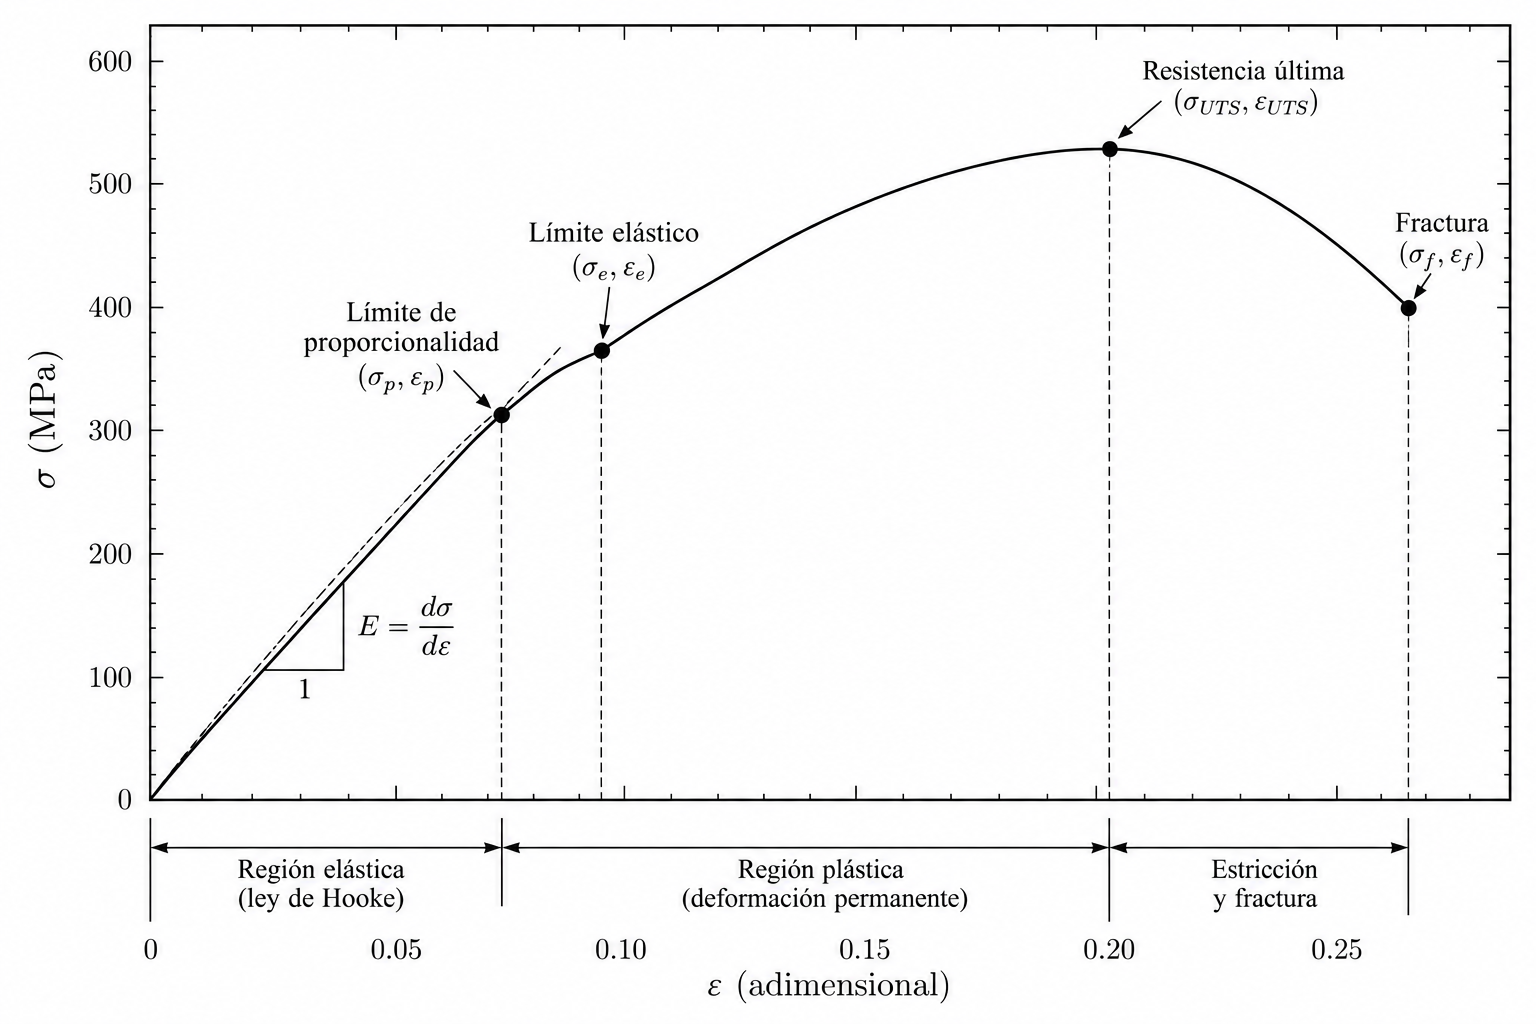
\includegraphics[width=0.90\textwidth]{../figuras/grafica1.png}
    \caption{Curva típica de esfuerzo--deformación para un material dúctil. Se indican el límite de proporcionalidad $(\sigma_p,\varepsilon_p)$, el límite elástico $(\sigma_e,\varepsilon_e)$, la resistencia última a la tracción $(\sigma_{\mathrm{UTS}},\varepsilon_{\mathrm{UTS}})$ y el punto de fractura $(\sigma_f,\varepsilon_f)$. La pendiente de la región lineal representa el módulo de Young $E$.}
    \label{fig:esfuerzo_deformacion}
\end{figure}

\par
\endgroup

\begingroup
\setlength{\leftskip}{1.5em}
\noindent
Dentro de la región elástica, al retirar la fuerza aplicada el cuerpo puede
recuperar su configuración inicial. Al superar el límite elástico pueden
producirse deformaciones permanentes, por lo que la trayectoria seguida por
el material deja de corresponder al comportamiento elástico ideal.


%------------------------------------------------
\subsection{Trabajo y energía de deformación}

Cuando una fuerza externa produce una deformación, realiza trabajo sobre el
sistema. Para una fuerza cuya magnitud depende de la deformación, el trabajo
realizado desde la posición inicial hasta una deformación $\Delta l$ se
expresa como

\[
W=\int_{0}^{\Delta l}F(x)\,dx.
\]

Por la ley de Hooke,

\[
W=\int_{0}^{\Delta l}kx\,dx,
\]

y al integrar,

\begin{equation}
\boxed{W=\frac{1}{2}k(\Delta l)^2}
\label{eq:trabajo_resorte}
\end{equation}

donde:

\begin{itemize}
    \item $W$: trabajo realizado para deformar el resorte, en $\mathrm{J}$.
\end{itemize}

Esta energía queda almacenada como energía potencial elástica mientras el
resorte permanece deformado. Gráficamente, el trabajo corresponde al área
bajo la curva $F$ frente a $\Delta l$. Para datos experimentales discretos,
esta área puede determinarse aproximadamente mediante integración numérica.


%------------------------------------------------
\subsection{Carga, descarga e histéresis}

En un sistema elástico ideal, la trayectoria seguida durante la aplicación
progresiva de una carga coincide con la trayectoria correspondiente a su
posterior retiro. Sin embargo, determinados materiales reales, como los
elastómeros, pueden presentar diferentes relaciones entre esfuerzo y
deformación durante los procesos de carga y descarga.

Cuando ambas trayectorias no coinciden se forma un ciclo de histéresis. El
trabajo realizado por unidad de volumen durante la deformación puede
expresarse como

\[
w=\int \sigma\,d\varepsilon.
\]

Por ello, la diferencia entre el trabajo realizado durante la carga y el
trabajo recuperado durante la descarga está asociada al área encerrada por
el ciclo esfuerzo--deformación:

\begin{equation}
\boxed{
w_{\mathrm{dis}}=
\oint \sigma\,d\varepsilon
}
\label{eq:histeresis}
\end{equation}

donde:

\begin{itemize}
    \item $w_{\mathrm{dis}}$: energía disipada por unidad de volumen,
    en $\mathrm{J/m^3}$.
\end{itemize}

En la presente experiencia, la comparación de las curvas de carga y descarga
permite analizar el grado de reversibilidad de la deformación del resorte y
de la liga, así como determinar experimentalmente la energía asociada al
ciclo de histéresis.
\par
\endgroup


\newpage
\section{Materiales y equipos}
\begingroup
\setlength{\leftskip}{1.5em}
\subsection{Elementos de montaje y soporte}

Elementos empleados para sostener los cuerpos elásticos y
aplicar las cargas durante la experiencia.

\begin{itemize}
    \item Soporte universal
    \item Elementos de sujeción
    \item Barra metálica
\end{itemize}


\subsection{Instrumentos de medición y adquisición de datos}

Instrumentos utilizados para determinar las magnitudes
experimentales y sus correspondientes incertidumbres.

\begin{itemize}
    \item Regla metálica: Incertidumbre instrumental de
    $\pm 0.5\,\mathrm{mm}$.

    \item Vernier: Incertidumbre instrumental de
    $\pm 0.02\,\mathrm{mm}$.

    \item Balanza: Incertidumbre instrumental de
    $\pm 0.5\,\mathrm{g}$.
\end{itemize}


\subsection{Componentes del sistema}

Elementos que constituyen los sistemas físicos sometidos
a deformación durante la experiencia.

\begin{itemize}
    \item Resorte helicoidal
    \item Liga elástica
    \item Cinco masas de distintos pesos
\end{itemize}

\begin{figure}[H]
    \centering
    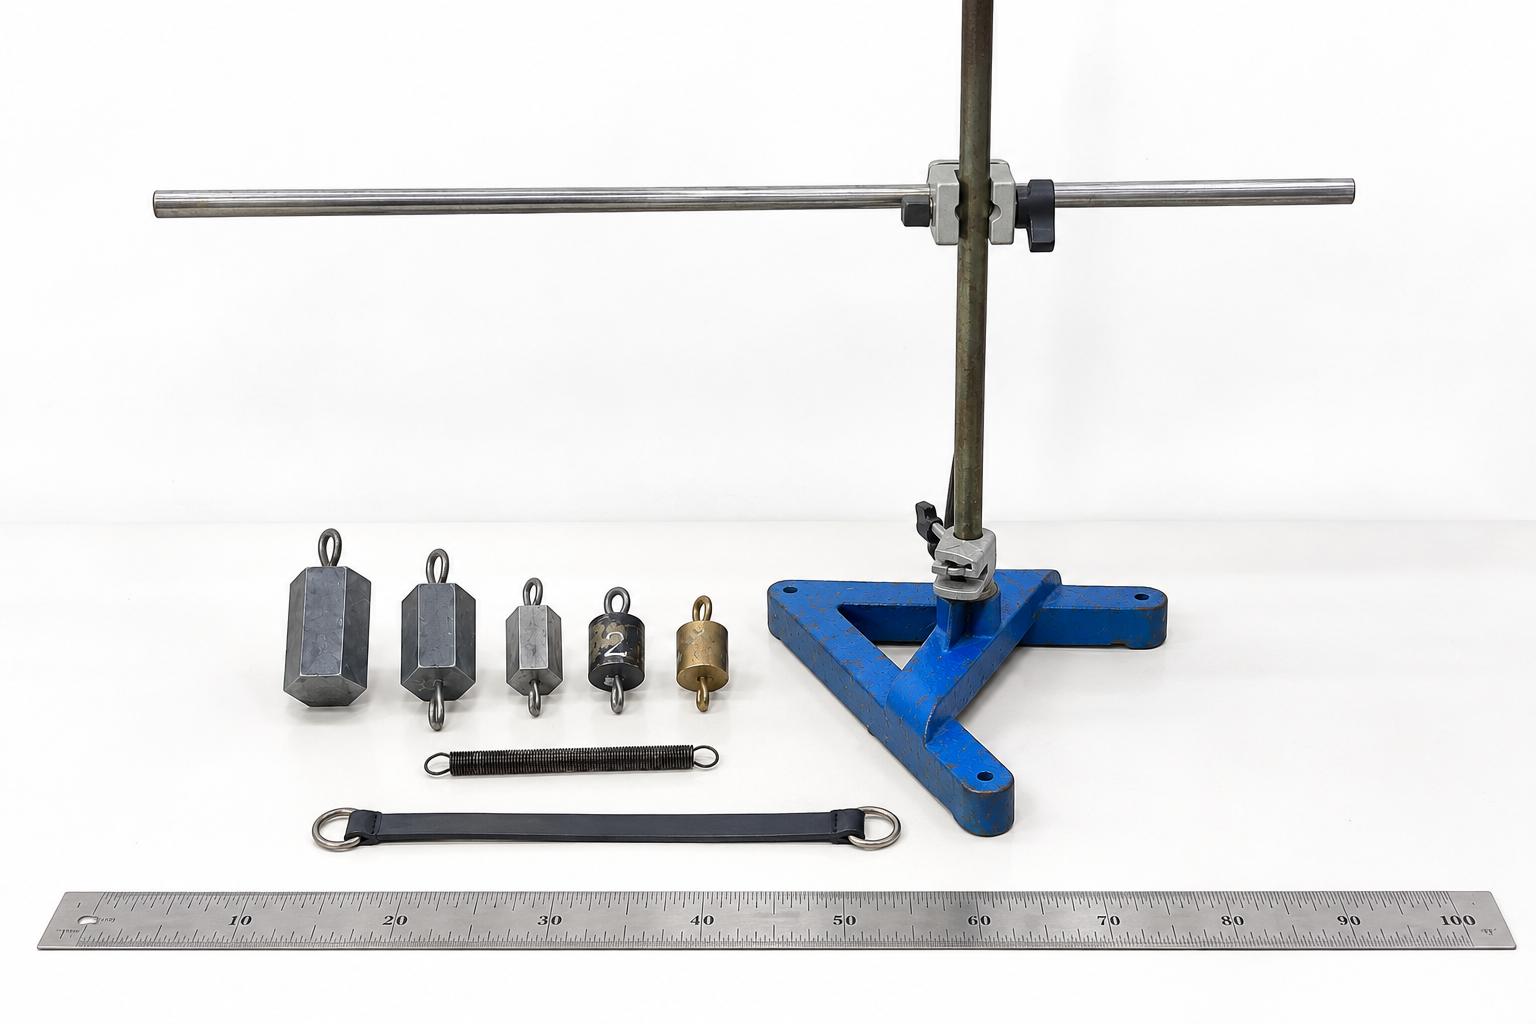
\includegraphics[width=0.90\textwidth]{../figuras/materiales_equipos.png}
    \caption{Equipo utilizado durante el proceso de experimenbtación.}
    \label{fig:materiales}
\end{figure}


\newpage
\section{Procedimiento experimental}

\begin{enumerate}

    \item En primera instancia, me encargué de medir las cinco
    masas con la balanza, mientras mi compañero preparaba el
    soporte universal y los instrumentos de medición.
    Posteriormente, registramos las dimensiones iniciales
    del resorte y de la liga.

    \item Suspendimos el resorte verticalmente del soporte
    universal y colocamos la primera masa. Una vez alcanzado
    el equilibrio, medimos su longitud con la regla
    milimetrada y su diámetro con el vernier.

    \item Añadimos progresivamente las cuatro masas restantes,
    sin retirar las anteriores, registrando las dimensiones
    del resorte en cada etapa. Observamos que su longitud
    aumentaba mientras su diámetro disminuía ligeramente.

    \item Después de alcanzar la carga máxima, retiramos las
    masas una por una, en orden inverso, y repetimos las
    mediciones de longitud y diámetro durante la descarga.

    \item Sustituimos el resorte por la liga elástica y
    repetimos el procedimiento de carga acumulativa.
    En cada etapa registramos su longitud, ancho y espesor,
    observando un alargamiento progresivo acompañado de
    una reducción de sus dimensiones transversales.

    \item Finalmente, retiramos las masas de la liga en orden
    inverso y registramos sus dimensiones durante la
    descarga. Organizamos los datos obtenidos en tablas
    para realizar posteriormente los cálculos y las
    gráficas correspondientes.

\end{enumerate}

\begin{figure}[H]
    \centering
    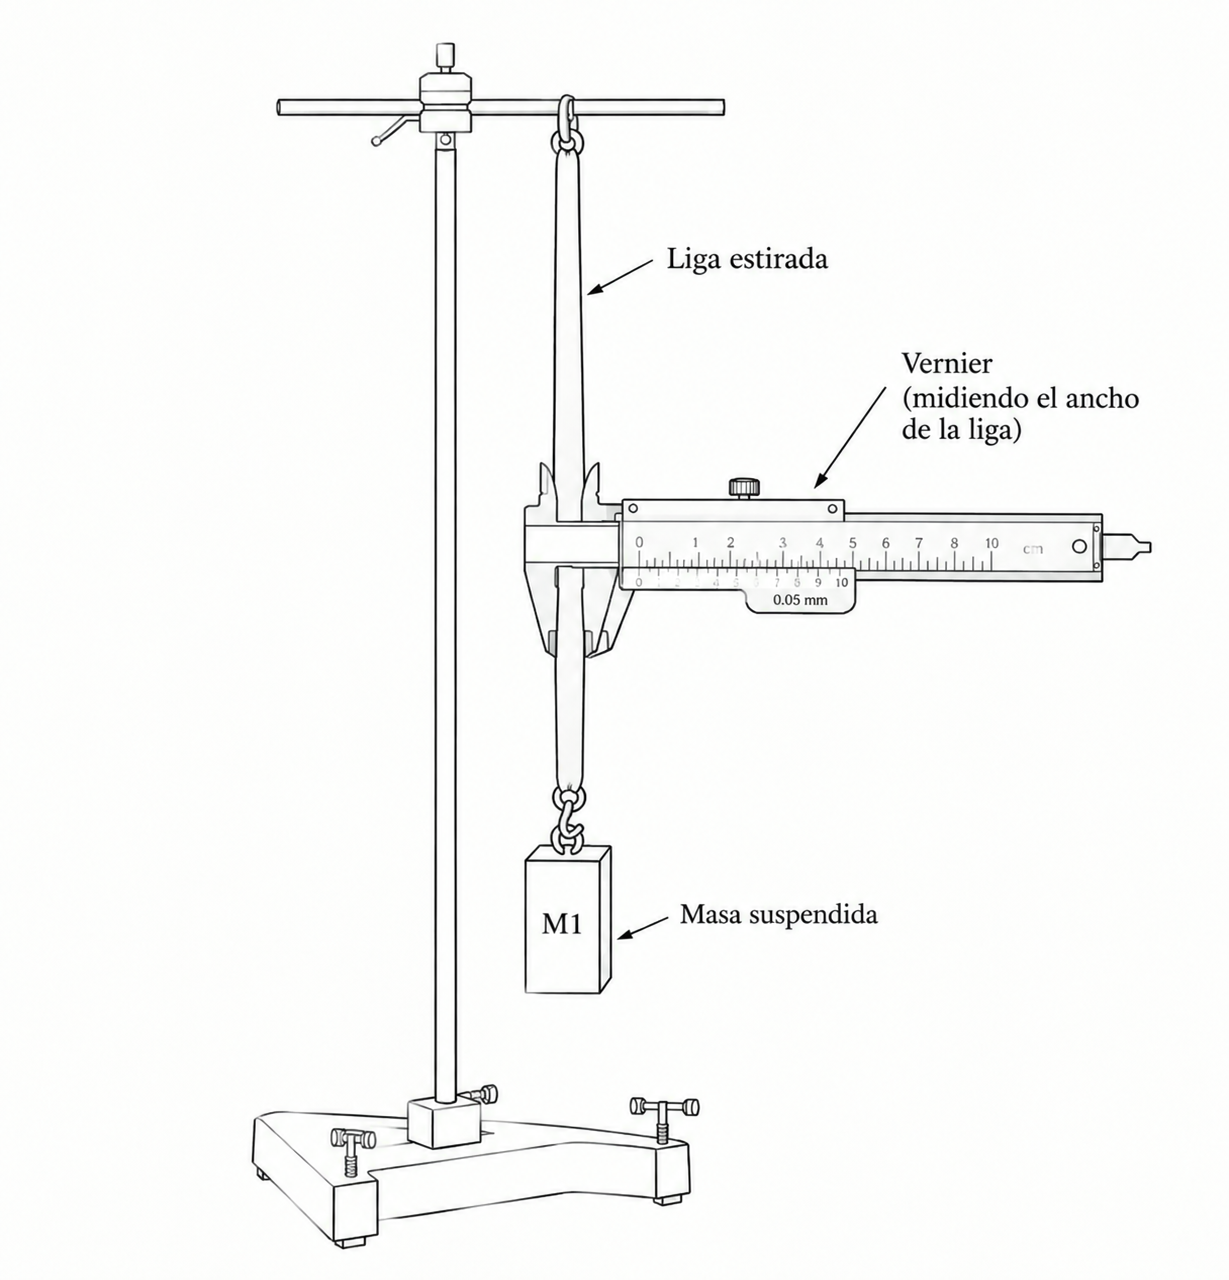
\includegraphics[width=0.75\textwidth]{../figuras/montaje.png}
    \caption{Ilustraci+on referencial de la medición del ancho
    de una liga elástica sometida a una carga mediante
    un vernier.}
    \label{fig:montaje_experimental}
\end{figure}


\newpage
\section{Datos experimentales}

En esta sección se presentan las mediciones realizadas durante
el estudio experimental de la ley de Hooke. Las incertidumbres instrumentales consideradas fueron
$\pm 0.0005\,\mathrm{m}$ para la regla milimetrada,
$\pm 0.00002\,\mathrm{m}$ para el vernier y
$\pm 0.0005\,\mathrm{kg}$ para la balanza.

\subsection{Medidas iniciales}
\begin{table}[H]
    \centering
    \small
    \renewcommand{\arraystretch}{1.15}
    \begin{tabular}{ccc}
        \toprule
        \textbf{Masa} &
        \textbf{$m$ (kg)} &
        \textbf{$u_m$ (kg)} \\
        \midrule
        $m_1$ & 0.148 & 0.00050 \\
        $m_2$ & 0.346 & 0.00050 \\
        $m_3$ & 0.596 & 0.00050 \\
        $m_4$ & 1.093 & 0.00050 \\
        $m_5$ & 2.081 & 0.00050 \\
        \bottomrule
    \end{tabular}
    \caption{Masas utilizadas para aplicar las cargas
    durante la experiencia.}
    \label{tab:masas_hooke}
\end{table}

\begin{table}[H]
    \centering
    \small
    \renewcommand{\arraystretch}{1.20}
    \setlength{\tabcolsep}{5pt}
    \begin{tabular}{lcc}
        \toprule
        \textbf{Magnitud} &
        \textbf{Resorte} &
        \textbf{Liga} \\
        \midrule
        Longitud inicial $\ell_0$ (m) &
        $0.2030 \pm 0.0005$ &
        $0.3320 \pm 0.0005$ \\

        Masa propia $m_0$ (kg) &
        $0.0463 \pm 0.0005$ &
        $0.0463 \pm 0.0005$ \\

        Diámetro inicial $d_0$ (m) &
        $0.01420 \pm 0.00002$ &
        --- \\

        Ancho inicial $a_0$ (m) &
        --- &
        $0.01480 \pm 0.00002$ \\

        Espesor inicial $b_0$ (m) &
        --- &
        $0.00675 \pm 0.00002$ \\
        \bottomrule
    \end{tabular}
    \caption{Magnitudes iniciales del resorte y de
    la liga.}
    \label{tab:dimensiones_iniciales}
\end{table}

\subsection{Mediciones del resorte helicoidal}

Se registraron las longitudes y los diámetros del resorte
para cinco condiciones de carga. Posteriormente, se
efectuaron las mediciones correspondientes al proceso
de descarga.

\begin{table}[H]
    \centering
    \small
    \renewcommand{\arraystretch}{1.12}
    \setlength{\tabcolsep}{7pt}
    \begin{tabular}{cccc}
        \toprule
        \textbf{Proceso} &
        \textbf{N°} &
        \textbf{$\ell$ (m)} &
        \textbf{$d$ (m)} \\
        \midrule
        Carga    & 1 & 0.204 & 0.01419 \\
        Carga    & 2 & 0.226 & 0.01418 \\
        Carga    & 3 & 0.272 & 0.01416 \\
        Carga    & 4 & 0.359 & 0.01415 \\
        Carga    & 5 & 0.532 & 0.01410 \\
        \midrule
        Descarga & 5 & 0.532 & 0.01410 \\
        Descarga & 4 & 0.359 & 0.01415 \\
        Descarga & 3 & 0.272 & 0.01416 \\
        Descarga & 2 & 0.226 & 0.01418 \\
        Descarga & 1 & 0.204 & 0.01419 \\
        \bottomrule
    \end{tabular}
    \caption{Mediciones experimentales de longitud
    y diámetro del resorte.}
    \label{tab:datos_resorte}
\end{table}

\noindent
Las incertidumbres de las mediciones del resorte fueron
$u_{\ell}=0.0005\,\mathrm{m}$ y
$u_d=0.00002\,\mathrm{m}$.

\subsection{Mediciones de la liga elástica}

Se midieron la longitud, el espesor y el ancho de la liga
para cada condición de carga y descarga. Estas mediciones
permitirán determinar posteriormente las deformaciones
longitudinales y las variaciones de su sección transversal.

\begin{table}[H]
    \centering
    \small
    \renewcommand{\arraystretch}{1.12}
    \setlength{\tabcolsep}{5pt}
    \begin{tabular}{ccccc}
        \toprule
        \textbf{Proceso} &
        \textbf{N°} &
        \textbf{$\ell$ (m)} &
        \textbf{$b$ (m)} &
        \textbf{$a$ (m)} \\
        \midrule
        Carga    & 1 & 0.340 & 0.00635 & 0.01480 \\
        Carga    & 2 & 0.352 & 0.00585 & 0.01410 \\
        Carga    & 3 & 0.373 & 0.00560 & 0.01330 \\
        Carga    & 4 & 0.437 & 0.00535 & 0.01215 \\
        Carga    & 5 & 0.584 & 0.00480 & 0.01060 \\
        \midrule
        Descarga & 5 & 0.584 & 0.00480 & 0.01060 \\
        Descarga & 4 & 0.437 & 0.00535 & 0.01215 \\
        Descarga & 3 & 0.373 & 0.00560 & 0.01330 \\
        Descarga & 2 & 0.352 & 0.00585 & 0.01410 \\
        Descarga & 1 & 0.340 & 0.00635 & 0.01480 \\
        \bottomrule
    \end{tabular}
    \caption{Mediciones experimentales de longitud,
    espesor y ancho de la liga.}
    \label{tab:datos_liga}
\end{table}

\noindent
Las incertidumbres instrumentales correspondientes
fueron $u_{\ell}=0.0005\,\mathrm{m}$,
$u_a=0.00002\,\mathrm{m}$ y
$u_b=0.00002\,\mathrm{m}$.

\par
\endgroup

\newpage
\section{Cálculos y resultados}

\subsection{En el resorte}
\subsubsection{Gráfica de la carga y descarga}

\begin{figure}[H]
    \centering
    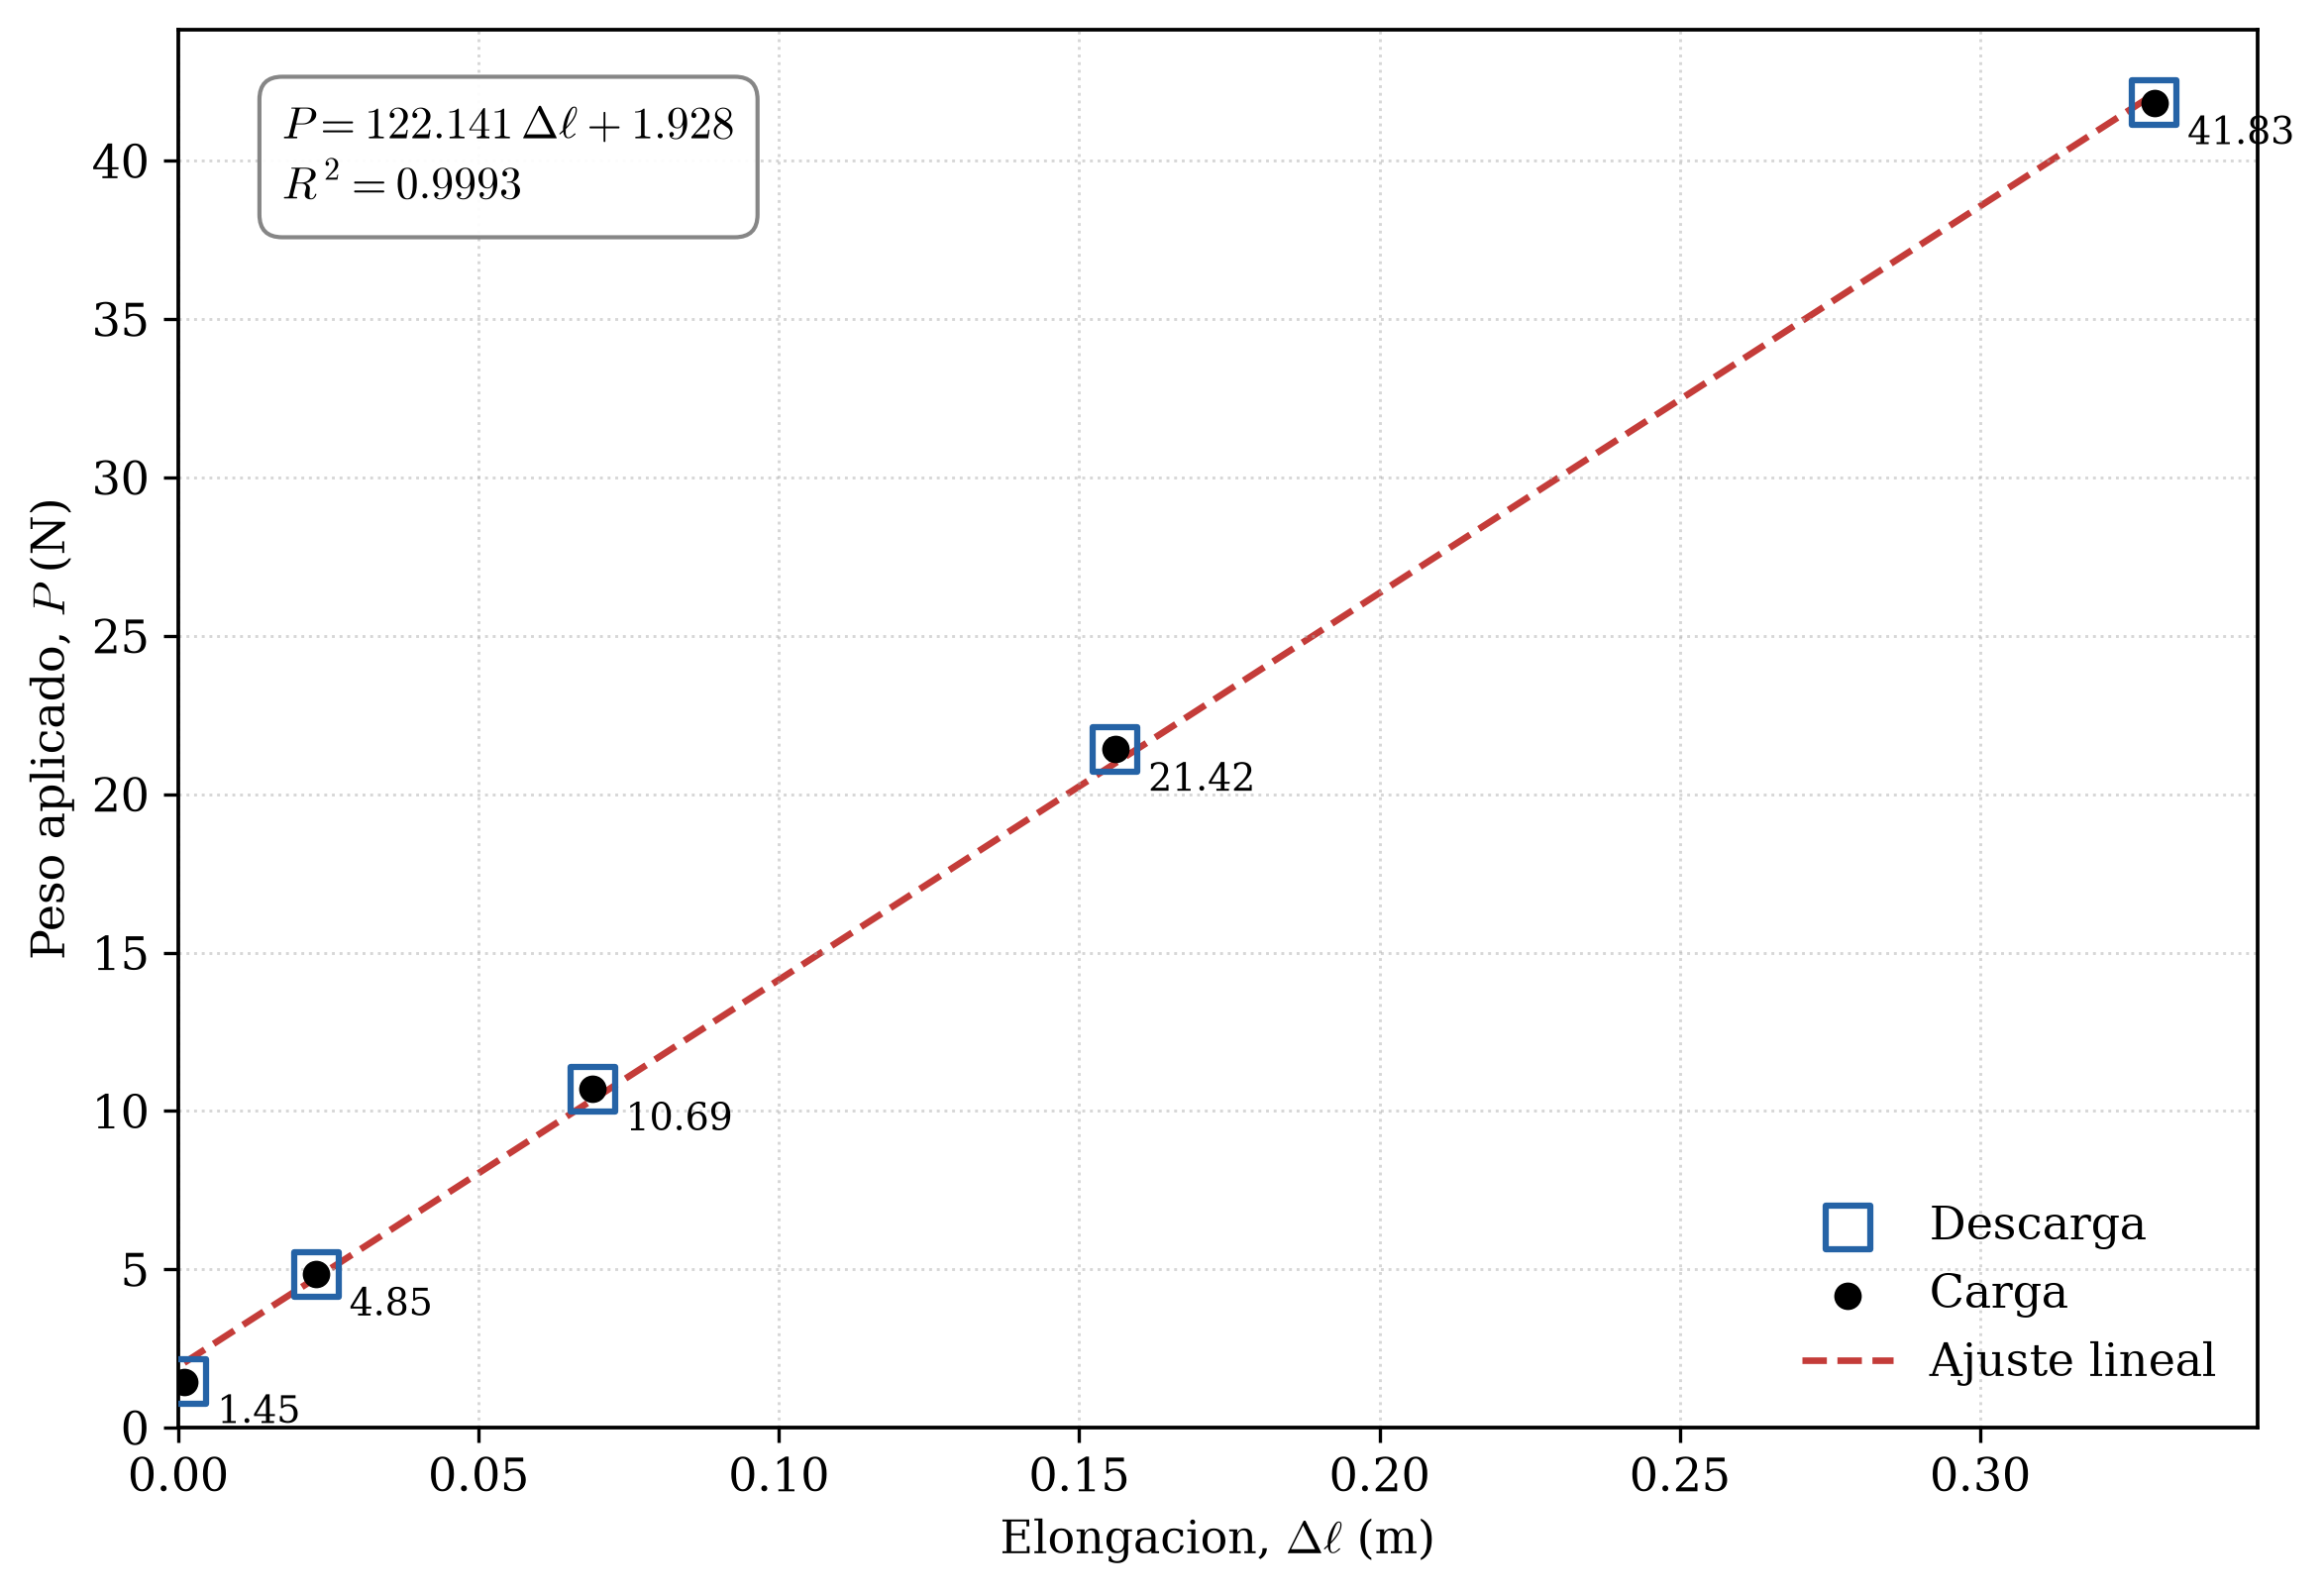
\includegraphics[width=0.85\textwidth]{../figuras/peso_elongacion_resorte.png}
    \caption{Relación entre $P$ y $\Delta\ell$ del resorte durante la carga y descarga.}
    \label{fig:peso_elongacion_resorte}
\end{figure}

\subsubsection{Gráfica del esfuerzo real versus deformación unitaria}

\begin{figure}[H]
    \centering
    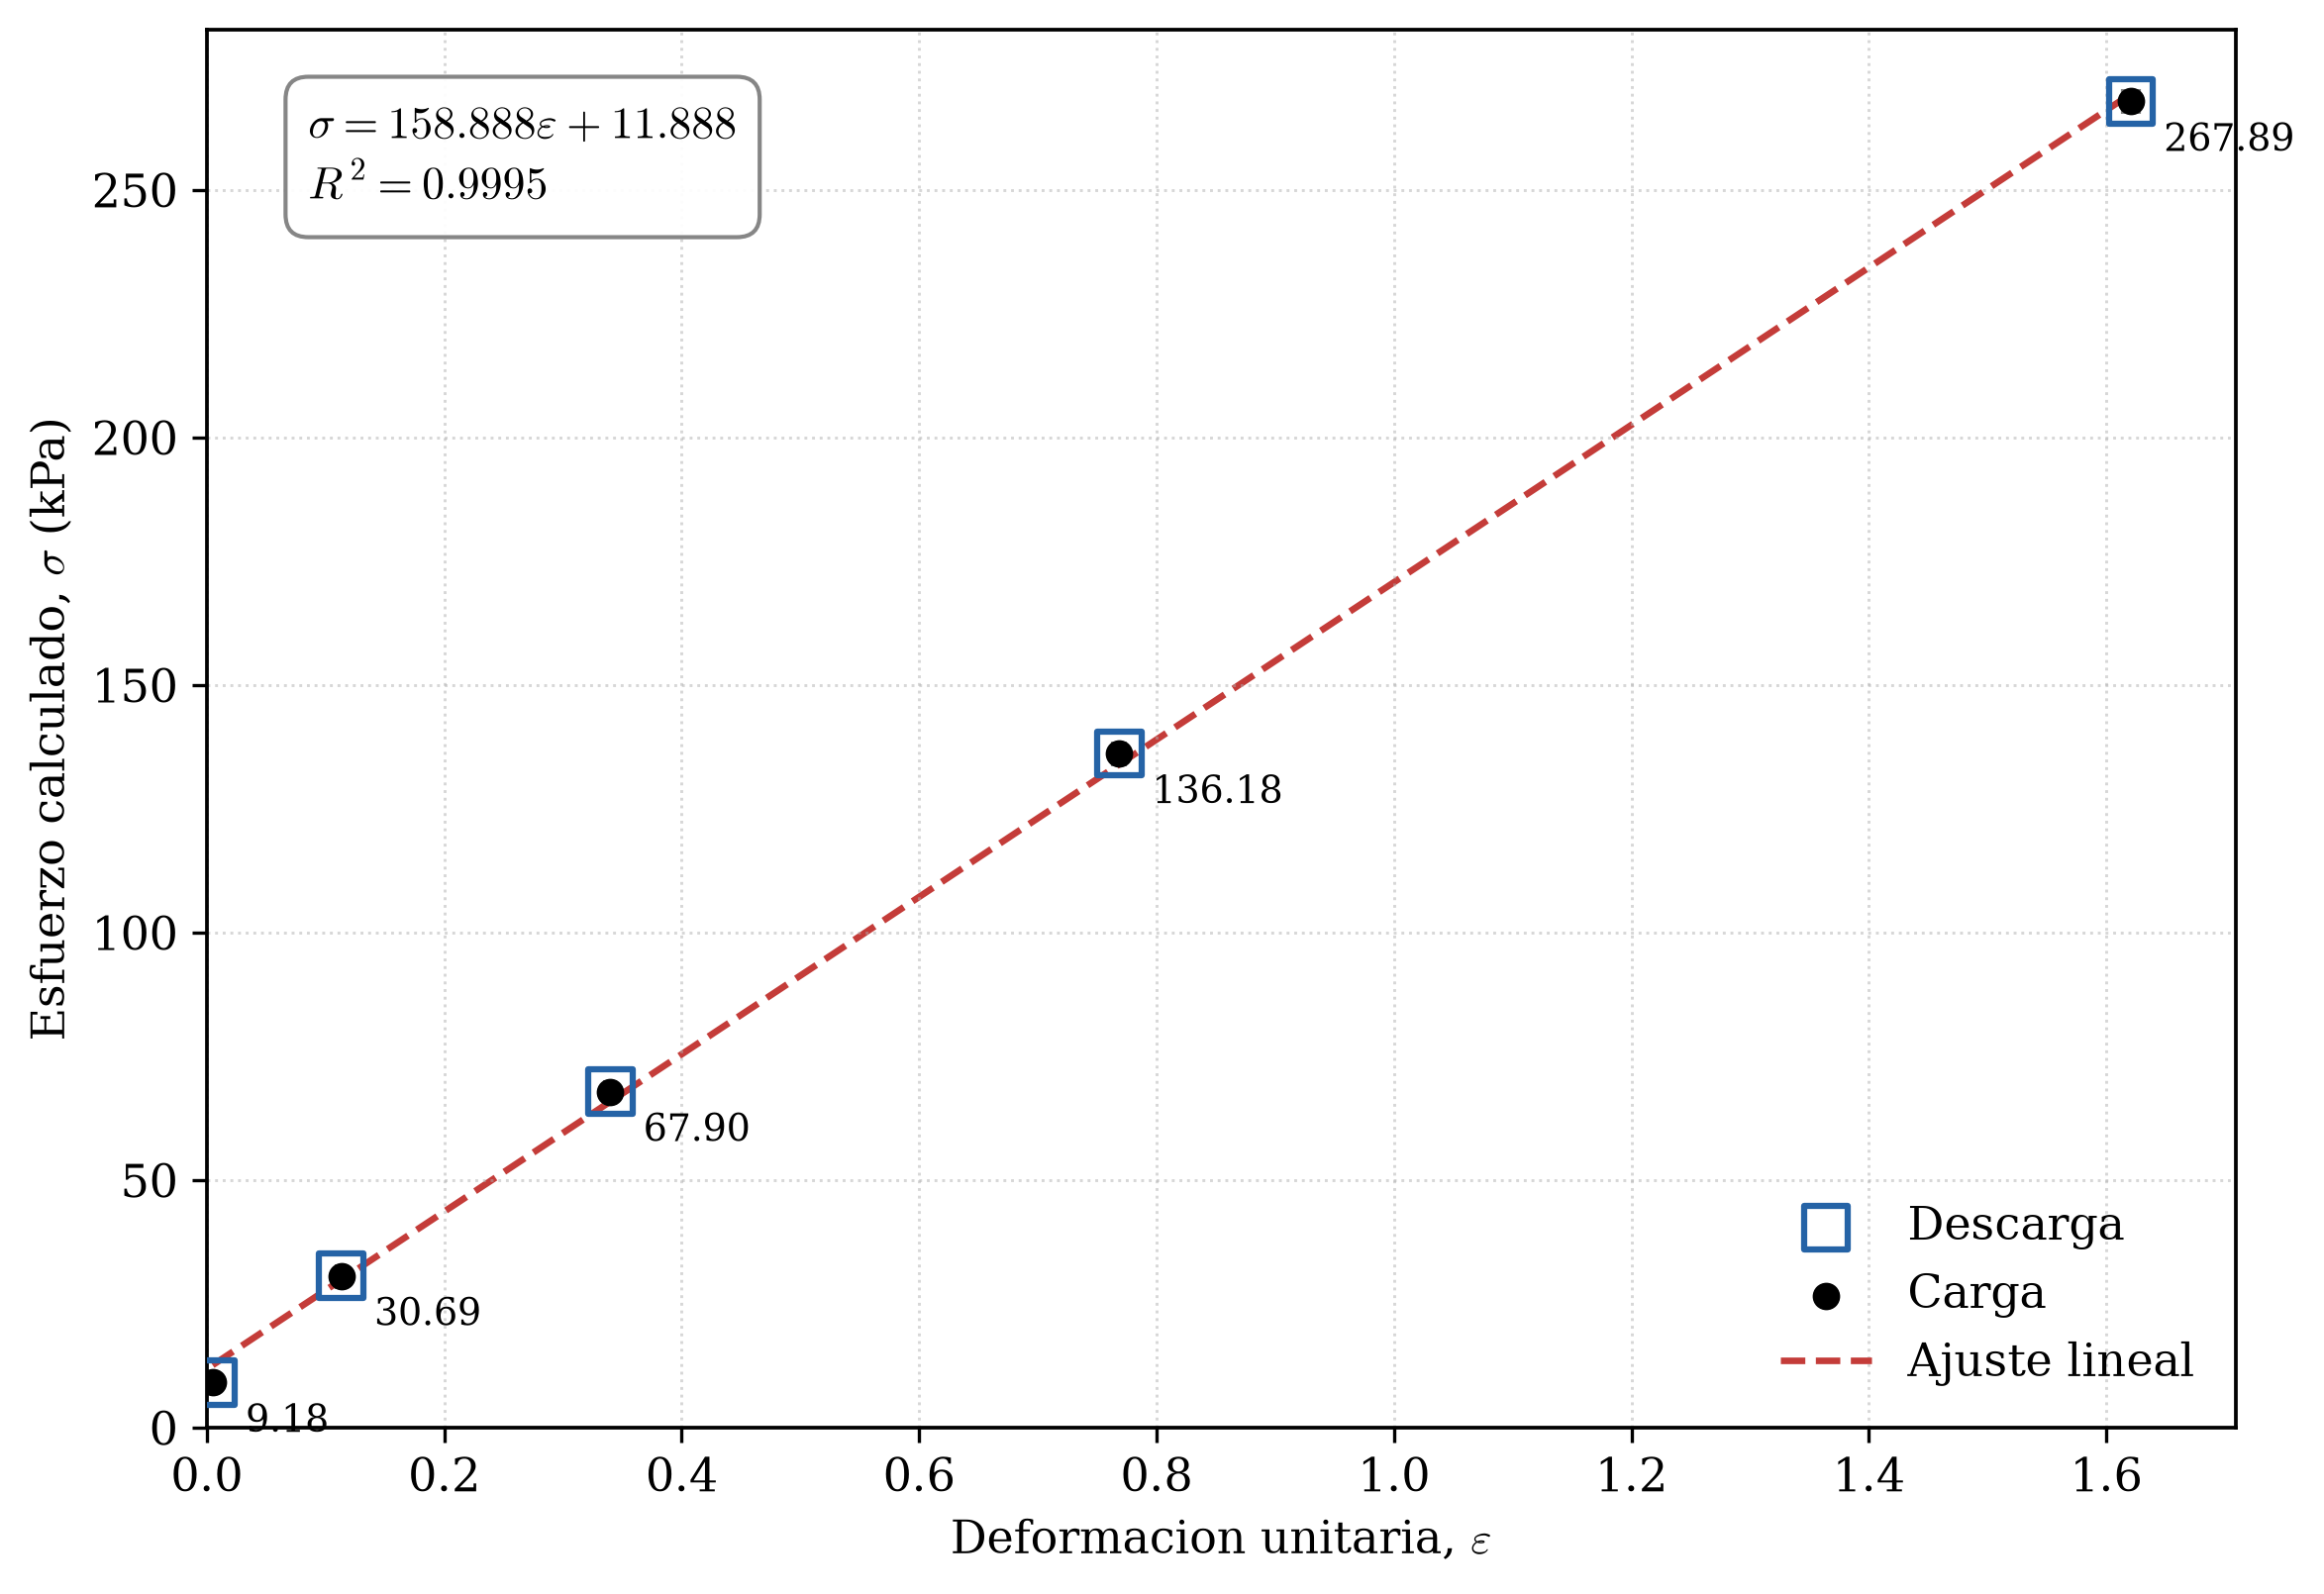
\includegraphics[width=0.85\textwidth]
    {../figuras/esfuerzo_deformacion_resorte.png}
    \caption{Relación entre $\sigma$ vs $\varepsilon$ de los procesos
    de carga y descarga.}
    \label{fig:esfuerzo_deformacion_resorte}
\end{figure}

\subsubsection{Análisis de las relaciones entre magnitudes físicas}

En respuesta a la pregunta \textit{«En cada gráfico, ¿qué relación
existe entre estas magnitudes?»}, planteada en la pág. 66 de
la guía de laboratorio, se analizaron las relaciones entre las
magnitudes experimentales mediante ajustes lineales por mínimos
cuadrados ordinarios, obteniéndose sus respectivas ecuaciones
y coeficientes de determinación ($R^2$).

\medskip

\noindent\textbf{a) Relación entre el peso aplicado
$P$ y la elongación $\Delta\ell$.}

En la Figura~\ref{fig:peso_elongacion_resorte} se observa que
el peso aplicado aumenta aproximadamente de manera lineal
con la elongación del resorte, en concordancia con el
comportamiento descrito por la ley de Hooke.


\begin{equation}
    \boxed{P = 122.141\,\Delta\ell + 1.928}
\end{equation}

\noindent
donde $P$ se expresa en newtons y $\Delta\ell$ en metros.
El coeficiente de determinación, $R^2 = 0.9993$, evidencia
una elevada correlación lineal entre ambas magnitudes.

La pendiente de la recta proporciona una estimación de
la constante elástica del resorte:

\begin{equation}
    k = 122.141\ \mathrm{N/m}.
\end{equation}

Sin embargo, el intercepto distinto de cero indica que
el ajuste experimental no reproduce exactamente la forma
ideal de la ley de Hooke, $P = k\Delta\ell$.

\medskip

\noindent\textbf{b) Relación entre el esfuerzo calculado
$\sigma$ y la deformación unitaria $\varepsilon$.}

En la Figura~\ref{fig:esfuerzo_deformacion_resorte} se
observa una relación aproximadamente lineal entre el
esfuerzo calculado y la deformación unitaria.

Los valores experimentales correspondientes a los procesos
de carga y descarga coinciden, por lo que ambas series
se superponen en la representación gráfica.

El ajuste lineal proporciona la siguiente ecuación:

\begin{equation}
    \boxed{\sigma = 158.888\,\varepsilon + 11.888}
\end{equation}

\noindent
donde $\sigma$ se expresa en kilopascales (kPa) y
$\varepsilon$ es una magnitud adimensional.

El coeficiente de determinación, $R^2 = 0.9995$,
indica que el modelo lineal describe adecuadamente
los datos experimentales.

No obstante, debido a que el esfuerzo se calculó
utilizando el área correspondiente al diámetro medido
del resorte helicoidal, la pendiente obtenida representa
una relación experimental aparente y no debe
identificarse directamente con el módulo de Young
del material.

En ambas representaciones se observa una marcada
tendencia lineal, compatible con el comportamiento
elástico del sistema dentro del intervalo de cargas
estudiado. Asimismo, la coincidencia de los puntos
experimentales de carga y descarga indica que no se
registraron diferencias entre ambos procesos con
la resolución de las mediciones realizadas.


\subsubsection{Determinación de la constante recuperadora
y del módulo de Young}

En respuesta a la pregunta planteada en la guía de
laboratorio, ¿Puede determinar, a partir de los gráficos, la constante recuperadora del resorte y el
módulo de Young? si eso es así, ¿cuál es el valor de Y? en caso contrario ¿explique cómo se
debería calcular?

De acuerdo con la ley de Hooke, la magnitud de la fuerza
elástica está relacionada con la elongación mediante:

\begin{equation}
    F = k\Delta\ell
\end{equation}

La ecuación experimental obtenida de la primera gráfica es:

\begin{equation}
    P = 122.141\,\Delta\ell + 1.928
\end{equation}

Al comparar ambas expresiones, se identifica que la
pendiente de la recta corresponde a la constante
recuperadora del resorte:

\begin{equation}
    k = \frac{dP}{d(\Delta\ell)}
\end{equation}

Por tanto:

\begin{equation}
    \boxed{k = 122.141\ \mathrm{N/m}}
\end{equation}

Este valor caracteriza la rigidez efectiva del resorte
dentro del intervalo de elongaciones estudiado.

\medskip

\noindent\textbf{Módulo de Young}

De la segunda gráfica, correspondiente al esfuerzo
calculado en función de la deformación unitaria,
se obtuvo la ecuación experimental:

\begin{equation}
    \sigma = 158.888\,\varepsilon + 11.888
\end{equation}

Para un material homogéneo sometido a tracción
uniaxial dentro de su régimen elástico, la ley
de Hooke establece:

\begin{equation}
    \sigma = Y\varepsilon
\end{equation}

Por comparación, la pendiente experimental es:

\begin{equation}
    \frac{d\sigma}{d\varepsilon}
    = 158.888\ \mathrm{kPa}
\end{equation}

Equivalentemente:

\begin{equation}
    \boxed{
    \frac{d\sigma}{d\varepsilon}
    = 1.58888\times10^{5}\ \mathrm{Pa}
    }
\end{equation}


\noindent\textbf{¿Es correcto ese valor?}

Matemáticamente sí, puesto que se obtiene directamente
de la pendiente de la recta de ajuste experimental.
Sin embargo, físicamente sabemos que el módulo de Young
de los materiales metálicos suele ser:

\begin{itemize}
    \item Acero: $Y \approx 2\times10^{11}\ \mathrm{Pa}$.
    \item Aluminio: $Y \approx 7\times10^{10}\ \mathrm{Pa}$.
\end{itemize}

El valor experimental obtenido,
$Y_{\mathrm{aparente}}=1.58888\times10^{5}\ \mathrm{Pa}$,
es considerablemente menor que estos valores de referencia.

Esta discrepancia puede deberse a factores que alteran la toma de medias durante el experimento, como medir directamente con una regla y estimar su longitud, algo que no es muy preciso.
Por tanto, el valor obtenido representa un módulo
aparente del resorte y no el módulo de Young
del material que lo constituye.


\subsubsection{Cálculo del trabajo realizado sobre el resorte}

El trabajo realizado por la fuerza externa durante la
deformación del resorte corresponde al área bajo la
curva del peso aplicado $P$ en función de la elongación
$\Delta\ell$. Para determinarlo hasta la tercera carga,
se empleó el método de integración numérica mediante
la regla del trapecio.

Los datos experimentales considerados son:

\begin{center}
\begin{tabular}{c c}
\hline
$\Delta\ell$ (m) & $P$ (N) \\
\hline
0.001 & 1.45188 \\
0.023 & 4.84614 \\
0.069 & 10.69290 \\
\hline
\end{tabular}
\end{center}

El trabajo se expresa mediante:

\begin{equation}
    W=\int_{0}^{\Delta\ell_3}P\,d(\Delta\ell).
\end{equation}

Para aplicar la regla del trapecio, se considera
adicionalmente el punto inicial
$(\Delta\ell_0,P_0)=(0,0)$.

En cada intervalo, el trabajo se aproxima mediante:

\begin{equation}
    W_i \approx
    \frac{P_i+P_{i+1}}{2}
    (\Delta\ell_{i+1}-\Delta\ell_i).
\end{equation}

\medskip

\noindent\textbf{Primer intervalo:}

\begin{equation}
    W_1=
    \frac{0+1.45188}{2}(0.001-0)
\end{equation}

\begin{equation}
    W_1\approx 0.000726\ \mathrm{J}.
\end{equation}

\medskip

\noindent\textbf{Segundo intervalo:}

\begin{equation}
    W_2=
    \frac{1.45188+4.84614}{2}
    (0.023-0.001)
\end{equation}

\begin{equation}
    W_2\approx 0.069278\ \mathrm{J}.
\end{equation}

\medskip

\noindent\textbf{Tercer intervalo:}

\begin{equation}
    W_3=
    \frac{4.84614+10.69290}{2}
    (0.069-0.023)
\end{equation}

\begin{equation}
    W_3\approx 0.357398\ \mathrm{J}.
\end{equation}

\medskip

\noindent\textbf{Trabajo total:}
\begin{align}
    W &= W_1+W_2+W_3 \\
      &\approx 0.000726+0.069278+0.357398.
\end{align}

Por tanto:

\begin{equation}
    \boxed{W\approx 0.4274\ \mathrm{J}}
\end{equation}


\subsection{En la liga elástica}

\subsubsection{Gráfica de la carga y descarga}

\begin{figure}[H]
    \centering
    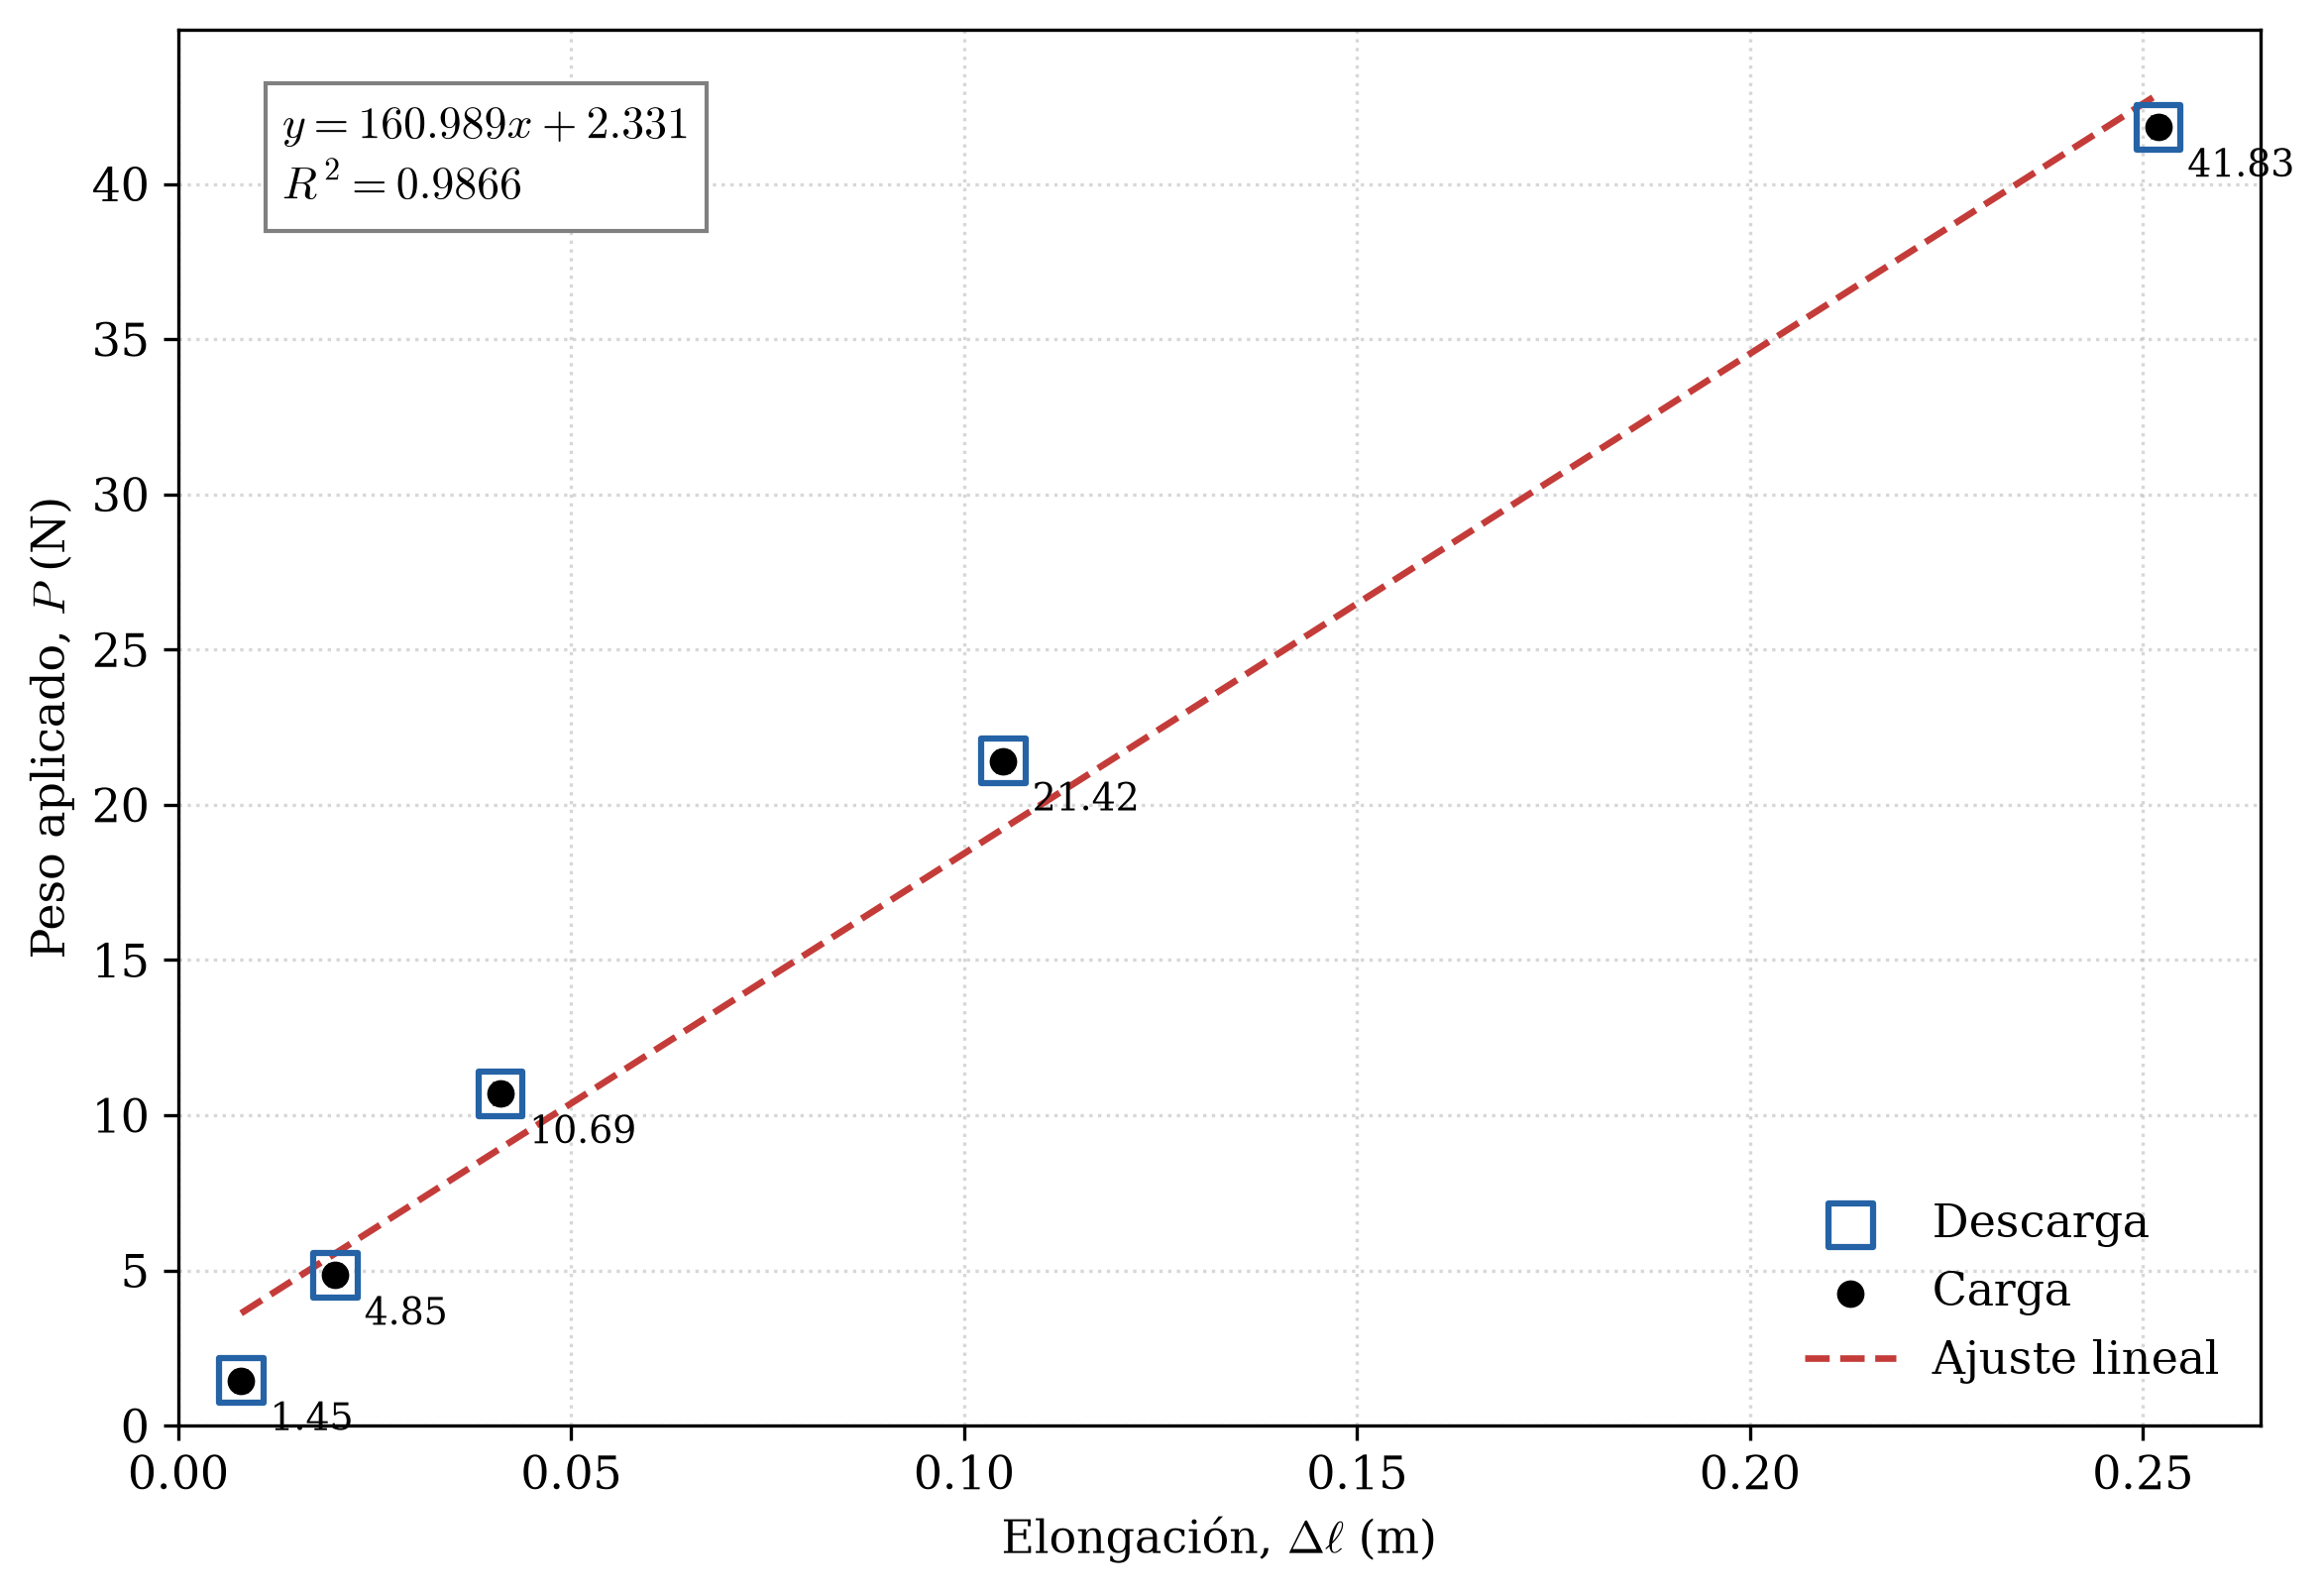
\includegraphics[width=0.85\textwidth]
    {../figuras/peso_elongacion_liga.png}
    \caption{Relación entre el peso aplicado $P$ y la
    elongación $\Delta\ell$ de la liga durante la
    carga y descarga.}
    \label{fig:peso_liga}
\end{figure}

\subsubsection{Gráfica del esfuerzo versus
deformación unitaria}

\begin{figure}[H]
    \centering
    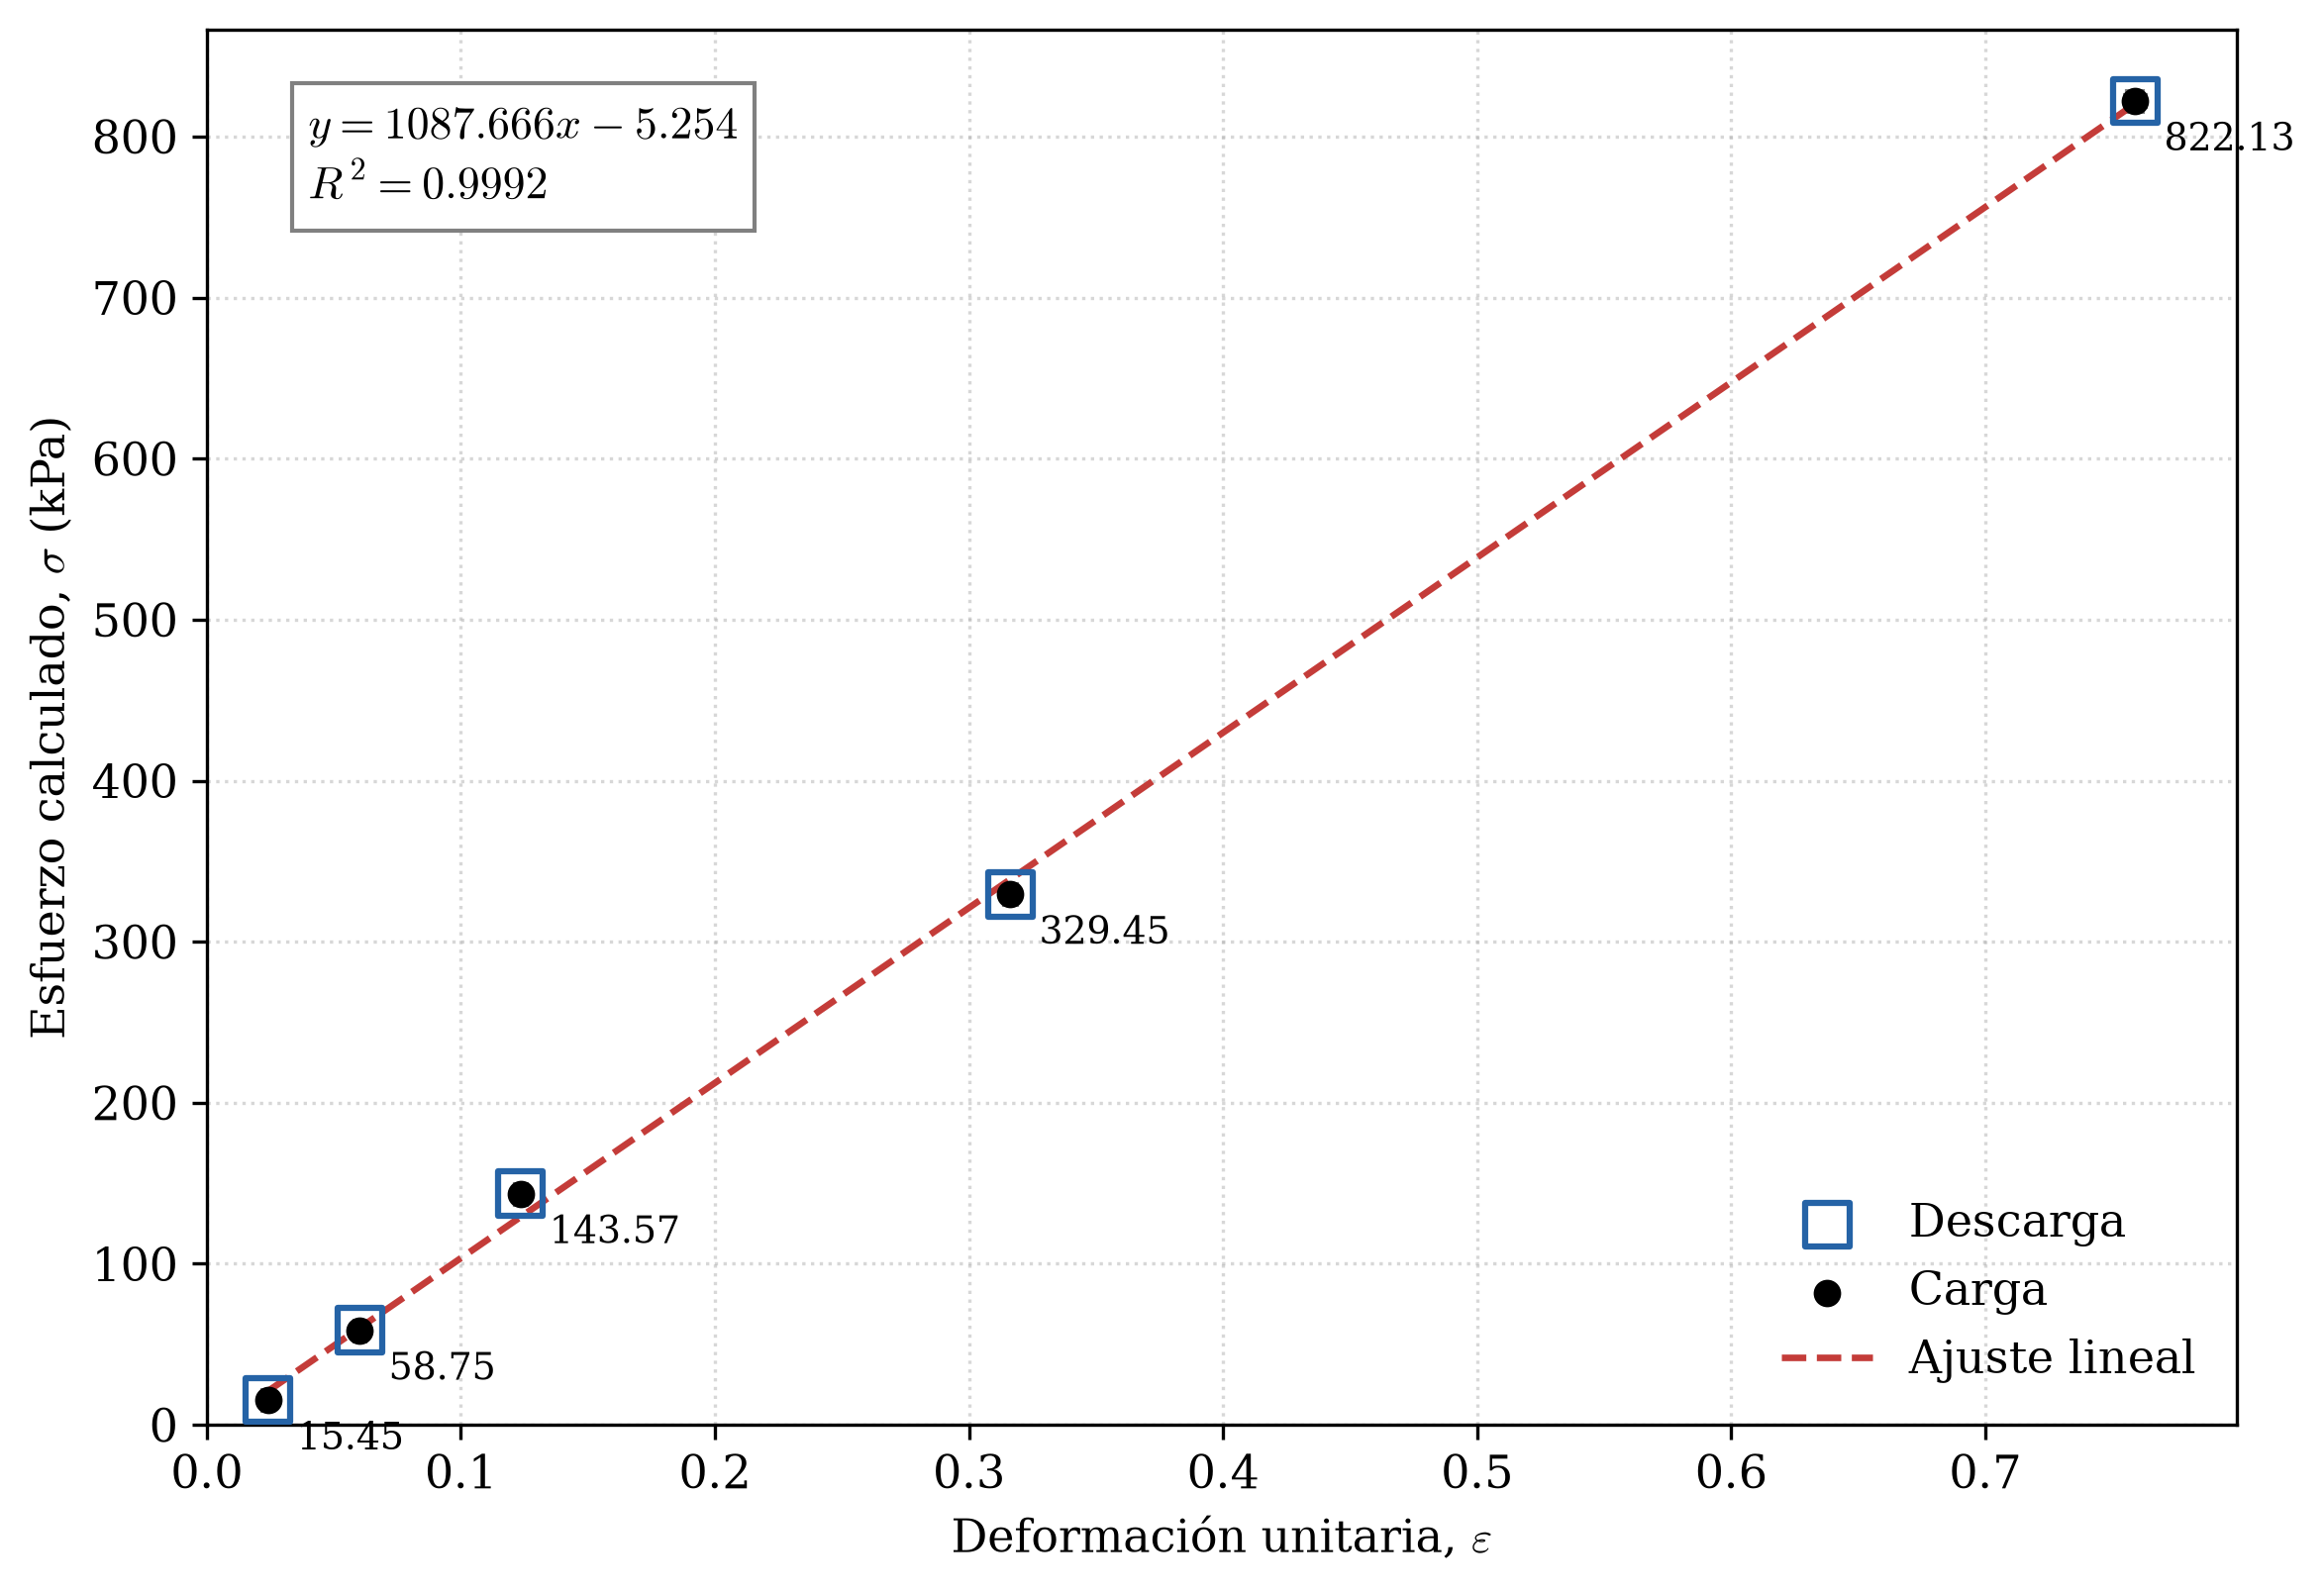
\includegraphics[width=0.85\textwidth]
    {../figuras/esfuerzo_deformacion_liga.png}
    \caption{Relación entre el esfuerzo calculado
    $\sigma$ y la deformación unitaria $\varepsilon$
    de la liga durante la carga y descarga.}
    \label{fig:esfuerzo_liga}
\end{figure}

\subsubsection{Interpretación del área encerrada
por la curva $\sigma$--$\varepsilon$}

En respuesta a la pregunta \textit{«En cada gráfico, ¿qué relación
existe entre estas magnitudes?»}, el área encerrada entre las curvas de carga y descarga
en el diagrama esfuerzo--deformación representa
la energía mecánica disipada por unidad de volumen
durante un ciclo de deformación, asociada al
comportamiento histerético del material.

Matemáticamente, se expresa como:

\begin{equation}
    w_{\mathrm{disipada}}
    = \oint \sigma\,d\varepsilon.
\end{equation}


\subsubsection{Determinación del área encerrada
por las curvas de carga y descarga}

Para determinar experimentalmente dicha área, se calcula:

\begin{equation}
    A =
    \left|
    \int_{\mathrm{carga}}\sigma\,d\varepsilon
    -
    \int_{\mathrm{descarga}}\sigma\,d\varepsilon
    \right|,
\end{equation}

Sin embargo, en el presente experimento, los valores
registrados para la carga y descarga coinciden,
por lo que ambas curvas se superponen en el
diagrama $\sigma$--$\varepsilon$.

En consecuencia, las áreas calculadas para ambos
procesos son iguales:

\begin{equation}
    A_{\mathrm{carga}}=A_{\mathrm{descarga}}.
\end{equation}

Por tanto:

\begin{equation}
    A =
    \left|A_{\mathrm{carga}}-A_{\mathrm{descarga}}\right|
    =0.
\end{equation}

Finalmente, la energía disipada por unidad de
volumen, calculada a partir de los datos disponibles,
es:

\begin{equation}
    \boxed{
    w_{\mathrm{disipada}}=0\ \mathrm{J/m^3}
    }
\end{equation}

\noindent\textbf{Interpretación física.}

La ausencia de un área de histéresis en la gráfica
puede estar relacionada con posibles errores
experimentales durante la toma de datos. Entre
ellos, se considera la realización apresurada de
las mediciones, la falta de tiempo de espera para
que la liga alcanzara una deformación estable y
las imprecisiones en la lectura de los instrumentos.

Asimismo, es posible que durante la descarga no
se hayan registrado con suficiente precisión las
pequeñas variaciones dimensionales del material.

Por tanto, el resultado obtenido no demuestra
la ausencia de disipación de energía, sino que
podría reflejar limitaciones en el procedimiento
experimental y en la precisión de las mediciones.


\subsubsection{Defina el esfuerzo de fluencia,
el esfuerzo límite y el módulo de elasticidad
en la tracción o compresión.}

\medskip

\noindent\textbf{Esfuerzo de fluencia ($\sigma_y$).}

Es el esfuerzo a partir del cual un material comienza
a experimentar deformaciones plásticas permanentes.
Al retirar la carga, el material ya no recupera
completamente su geometría original.

\medskip

\noindent\textbf{Esfuerzo límite ($\sigma_u$).}

Es el máximo esfuerzo nominal que un material puede
soportar durante un ensayo de tracción antes de que
se produzca una disminución de su capacidad resistente.
Se conoce también como resistencia última a la tracción.

\medskip

\noindent\textbf{Módulo de elasticidad ($Y$).}

Es una propiedad mecánica que cuantifica la rigidez
de un material sometido a tracción o compresión
uniaxial. En el régimen elástico lineal, se define
como la relación entre el esfuerzo normal y la
deformación longitudinal:

\begin{equation}
    \boxed{Y=\frac{\sigma}{\varepsilon}}
\end{equation}

Su unidad en el Sistema Internacional es el pascal
($\mathrm{Pa}$).

\subsubsection{¿Qué entiende por esfuerzo normal?
¿Existe diferencia entre un esfuerzo tangencial
y un esfuerzo de torsión?}

El esfuerzo normal ($\sigma$) es la fuerza interna
por unidad de área que actúa perpendicularmente
a una sección transversal del material:

\begin{equation}
    \boxed{\sigma=\frac{F_{\perp}}{A}}
\end{equation}

Puede producir deformaciones de tracción o compresión.

El esfuerzo tangencial ($\tau$), también denominado
esfuerzo cortante, corresponde a la componente
de la fuerza interna que actúa paralelamente
a una superficie:

\begin{equation}
    \boxed{\tau=\frac{F_{\parallel}}{A}}
\end{equation}

Por su parte, la torsión es una solicitación mecánica
producida por la aplicación de un momento de fuerza
alrededor del eje longitudinal de un cuerpo.
Esta genera esfuerzos cortantes distribuidos
sobre sus secciones transversales.

Por tanto, existe una diferencia conceptual:
el esfuerzo tangencial es una componente del estado
de esfuerzos, mientras que la torsión es un tipo
de carga que produce esfuerzos tangenciales.

\newpage
\section{Conclusiones}

\begin{enumerate}
    \item El resorte presentó una relación aproximadamente
    lineal entre el peso aplicado y la elongación,
    obteniéndose una constante elástica experimental
    de $k=122.141\ \mathrm{N/m}$ mediante regresión
    lineal, con un coeficiente de determinación
    $R^2=0.9993$.

    \item La gráfica del esfuerzo calculado frente
    a la deformación unitaria del resorte también
    presentó una elevada correlación lineal.
    Sin embargo, la pendiente obtenida no representa
    directamente el módulo de Young del material,
    debido a la geometría helicoidal del sistema.

    \item En la liga elástica se observó un incremento
    del peso aplicado con la elongación, aunque
    su respuesta mecánica difiere de la del resorte.
    El ajuste lineal de la relación peso--elongación
    presentó un coeficiente de determinación
    $R^2\approx0.9866$.

    \item Las curvas de carga y descarga de la liga
    coincidieron con los datos registrados, por lo
    que no se obtuvo un área de histéresis medible.
    Esta observación podría estar relacionada con
    limitaciones experimentales, como mediciones
    apresuradas, imprecisiones instrumentales
    o tiempos insuficientes de estabilización
    durante la descarga.

    \item Finalmente, se comprobó la utilidad
    del análisis gráfico, la regresión lineal
    y la integración numérica para caracterizar
    experimentalmente el comportamiento mecánico
    de sistemas elásticos y evaluar las limitaciones
    de los resultados obtenidos.
\end{enumerate}

\newpage

\begin{thebibliography}{99}

\bibitem{serway}
Serway, R. A. y Jewett, J. W.
\textit{Física para ciencias e ingeniería}.
Volumen 1. Cengage Learning.

\bibitem{sears}
Young, H. D. y Freedman, R. A.
\textit{Física universitaria}.
Volumen 1. Pearson Educación.

\bibitem{halliday}
Halliday, D., Resnick, R. y Walker, J.
\textit{Fundamentos de física}.
Wiley.

\bibitem{giancoli}
Giancoli, D. C.
\textit{Física: principios con aplicaciones}.
Pearson Educación.

\bibitem{guia}
Universidad Nacional de Ingeniería.
\textit{Guía de laboratorio de Física II:
Ley de Hooke}.
Facultad de Ciencias.

\end{thebibliography}

\newpage

% ==========================================
% ANEXOS
% ==========================================

\newpage
\section{Anexos}

\subsection{Repositorio del proyecto}

Los códigos utilizados para el procesamiento de
datos experimentales, la elaboración de las gráficas
y los archivos fuente del informe se encuentran
disponibles en el siguiente repositorio:

\begin{center}
    \url{https://github.com/USUARIO/REPOSITORIO}
\end{center}

\subsection{Participación de los integrantes}

La distribución de responsabilidades del equipo
se presenta en la Tabla~\ref{tab:participacion}.

\begin{table}[H]
    \centering
    \label{tab:participacion}
    \renewcommand{\arraystretch}{1.4}
    \small

    \begin{tabular}{|p{3.7cm}|p{1.7cm}|p{7.1cm}|}
        \hline
        \textbf{Apellidos y nombres} &
        \textbf{Código} &
        \textbf{Responsabilidades} \\
        \hline

        Moreno Cabanillas, Alexandra Romina &
        20251764F &
        Análisis de resultados y redacción
        del informe. \\
        \hline

        Polak Mory, Mauricio Andre &
        20250575E &
        Procesamiento de datos experimentales,
        cálculos experimentales y análisis
        de resultados. \\
        \hline

        Cárdenas Loyola, Pablo Mauro &
        20262378E &
        Elaboración de gráficas,registro y verificación de datos,
        análisis de incertidumbres. \\
        \hline

    \end{tabular}
\end{table}

Los tres integrantes participaron en la ejecución
de la experiencia, la discusión de los resultados
y la revisión general del informe.


\end{document}